\documentclass[]{../template/Report}%方括号内写yuxi即生成预习报告\documentclass[yuxi]{../template/Report}
\settemplatedir{../template/}%设置模板路径
\sisetup{
    separate-uncertainty = true,
    per-mode = symbol
}

\exname{固定均匀弦振动的研究} %实验名称
\extable{} %实验桌号
\instructor{} %指导教师
\class{} %班级
\name{} %姓名
\stuid{} %学号

\nyear{} %年
\nmonth{} %月
\nday{} %日
\nweekday{} %星期几，e.g. \nweekday{三}
\daypart{}%上午/下午

\redate{} %如有实验补做，补做日期
\resitu{} %情况说明：

\begin{document}
\maketitle%输出封面

\section{预习报告（10分）}
（注：将已经写好的“物理实验预习报告”内容拷贝过来）

\subsection{实验综述（5分）}
（自述实验现象、实验原理和实验方法，包括必要的光路图、电路图、公式等。不超过500字。）
\subsubsection{实验步骤}
1）固定频率，调节位置
\par
2）固定位置，调节频率
\par
3）保持张力、频率一定，测量波长与质量。
\par
4）保持张力不变，改变频率大小，测量波长。
\par
5）保持频率不变，改变张力大小，测量波长。
\par
6）计算 v，线性回归得到$\rho $，且进行不确定度分析。


\subsubsection{实验原理}
\textbf{(1)驻波}
\par
入射波和反射波这两列同领率的波在同一弦上沿相反方同传播时产生干涉，调节支撑点距离到适当位置，弦线上会形成驻波(如图)
\begin{figure}[H]
    \centering
    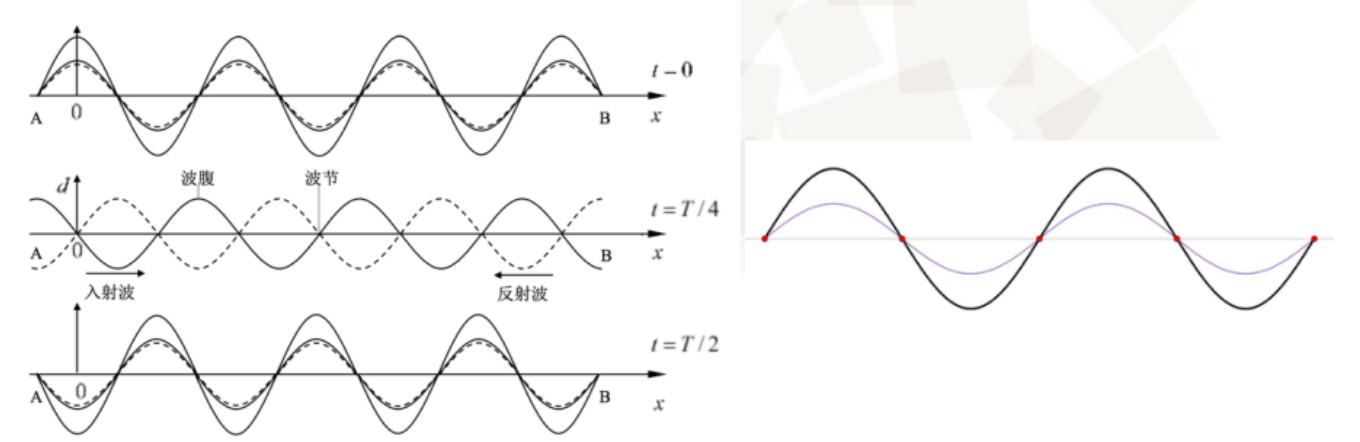
\includegraphics[width=0.6\textwidth]{figures/实验原理_驻波.png}
    \caption{驻波形成示意图}
\end{figure}
\begin{figure}[H]
    \centering
    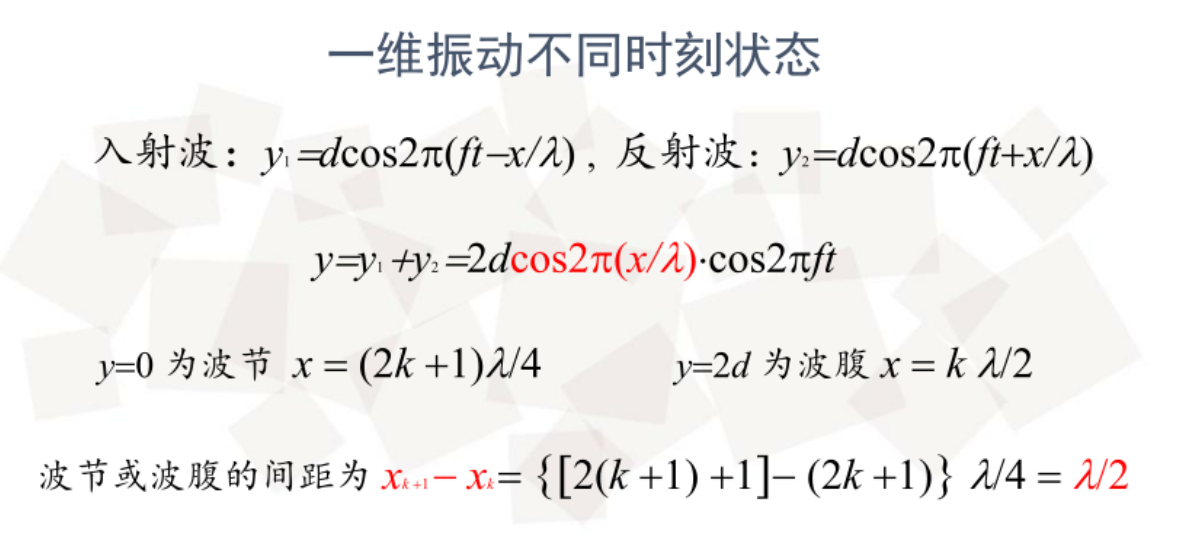
\includegraphics[width=0.6\textwidth]{figures/一维振动不同时刻状态.png}
    \caption{一维振动不同时刻状态}
\end{figure}

\textbf{(2)基础公式——应力、应变与模量(包括杨氏模量、剪切模量等)}
\par
2.1 在材料弹性限度范围内，模量 = 应力 / 应变
\par
2.2 正应力 = 作用力 / 垂直作用面积
\par
2.3 剪切应力 = 作用力 / 平行作用面积
\par
2.4 应变 = 形变量 / 原尺寸

\textbf{(3)一维波动方程推导}
\begin{figure}[H]
    \centering
    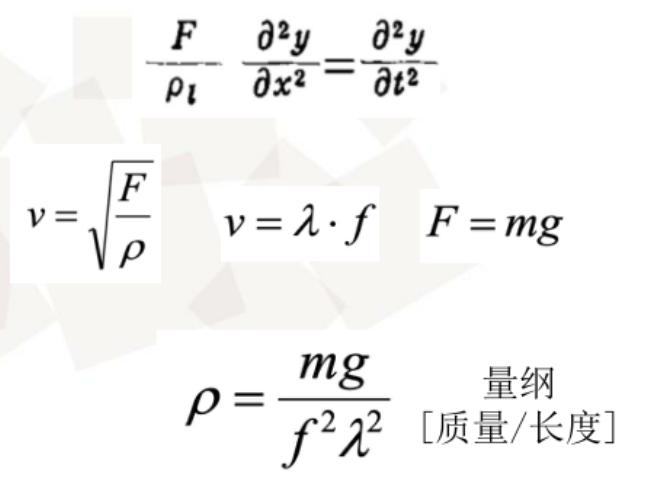
\includegraphics[width=0.5\textwidth]{figures/波动方程推导.png}
    \caption{一维波动方程推导}
\end{figure}

\subsection{实验重点（3分）}
（简述本实验的学习重点，不超过100字。）
\par
(1)\textbf{观察固定弦振动传播时形成的横驻波}
\par
(2)\textbf{了解振动在弦上传播的规律：}
\par
(3)\textbf{改变频率或弦张力测算均匀弦上横波传播速度v及弦线密度ρ}



\subsection{实验难点（2分）}
（简述本实验的实现难点，不超过100字。）
\par
(1)\textbf{驻波的稳定形成与调节：}需同时控制振动频率、弦线张力（通过砝码质量调节）和弦长（振动源与固定端距离）三个变量，使弦上形成清晰、稳定的驻波。三者会相互影响，例如张力过小时驻波易受外界干扰抖动，频率过高时波节密集难以分辨，通常需要反复调试才能找到稳定状态。
\par
(2)\textbf{波节位置的准确判断：}驻波波节处理论上振幅为零，但实际中因弦线弹性形变等因素，波节并非绝对静止，而是存在微小振动。需通过多次观察确定“振幅最小点”，尤其当波节靠近振动源或固定端时，易与边缘效应混淆，导致波长（相邻波节距离的2倍）测量偏差。
\par
(3)\textbf{张力与频率的精确控制：}滑轮存在摩擦时，实际张力小于砝码重力；信号发生器输出频率若波动，会使驻波“漂移”，需实时监测频率显示并微调。
\par
(4)\textbf{外界环境干扰：}实验台震动、气流扰动或周围噪音会导致弦线额外抖动，使波节模糊。需在操作时保持环境稳定（如避免触碰实验台），但实际中完全消除干扰较难，易影响数据重复性。
\par

\begin{fullreportonly}
\section{原始数据（20分）}
（将有老师签名的“自备数据记录草稿纸”的扫描或手机拍摄图粘贴在下方，完整保留姓名，学号，教师签字和日期。）
% \begin{figure}[H]
%     \centering
%     
\includegraphics[width=0.6\textwidth]{figures/原始数据.jpg}
%     \caption{原始数据}
% \end{figure}

\section{结果与分析（60分）}
\subsection{数据处理与结果（30分）}
（列出数据表格、选择适合的数据处理方法、写出测量或计算结果。） \\
砝码盘的质量 M = 5.055g $\quad$ 重力加速度 g = 9.793 $m/s^2$
\subsubsection{实验一：固定张力，改变频率}
测量弦线的质量线密度$\rho$ 及横波的速度 u。
\par
核心公式：波速 $u = \lambda \times f$ \quad 质量线密度$\rho = \frac{F}{u^2} = \frac{F}{f^2\lambda^2}$
\par
\begin{table}[H]
    \centering
    \caption{实验一固定F，改变f}
    \begin{tabular}{|c|c|c|c|c|c|c|}
        \hline
        \multicolumn{7}{|c|}{$F = (40 + M) \times 10^{-3} \times 9.793 = 0.441$（N）}  \\
        \hline
        \textbf{频率f(Hz)} & \textbf{驻波段数n} & \textbf{$L_\text{中}$(cm)} & \textbf{$L_\textbf{右}$(cm)} & \textbf{$\frac{|L_\textbf{右} - L_\textbf{左}|}{n}$(cm)} & \textbf{波长$\lambda$(cm)} & \textbf{质量线密度$\rho$(kg/m)}  \\
        \hline
        60 & 2 & 45.58 & 94.32 & 48.74 & 97.48 & 1.289$\times 10^{-4}$  \\
        \hline
        80 & 2 & 35.46 & 72.16 & 36.70 & 73.40 & 1.279$\times 10^{-4}$  \\
        \hline
        100 & 2 & 29.28 & 58.94 & 29.66 & 59.32 & 1.253$\times 10^{-4}$  \\
        \hline
        120 & 2 & 24.28 & 49.42 & 25.14 & 50.28 & 1.211$\times 10^{-4}$  \\
        \hline
        140 & 2 & 20.76 & 41.68 & 20.92 & 41.84 & 1.285$\times 10^{-4}$  \\
        \hline
        160 & 2 & 18.40 & 36.72 & 18.32 & 36.64 & 1.283$\times 10^{-4}$  \\
        \hline
        \multicolumn{2}{|c|}{\textbf{质量线密度平均值$\bar \rho$(kg/m)}} & 1.267 &
        \multicolumn{3}{|c|}{\textbf{质量线密度离散度$\Delta \rho$(kg/m)}} & 0.030  \\
        \hline
    \end{tabular}
\end{table}
求得质量线密度 $\rho = (1.267 \pm 0.030) \times 10^{-4}$(kg/m)

\subsubsection{实验二：固定频率，改变张力}
\begin{table}[H]
    \centering
    \caption{实验二固定f，改变F}
    \begin{tabular}{|c|c|c|c|c|c|c|}
        \hline
        \multicolumn{7}{|c|}{\textbf{频率f = 80Hz}}  \\
        \hline
        \textbf{张力F(N)} & \textbf{驻波段数n} & \textbf{$L_\text{中}$(cm)} & \textbf{$L_\textbf{右}$(cm)} & \textbf{$\frac{|L_\textbf{右} - L_\textbf{左}|}{n}$(cm)} & \textbf{波速u(cm/s)} & \textbf{$u^2$(${cm}^2/s^2$)}  \\
        \hline
        (M+25)g=0.294 & 2 & 29.40 & 59.40 & 30.00 & 4800 & 2.304$\times 10^7$  \\
        \hline
        (M+30)g=0.343 & 2 & 31.31 & 64.21 & 32.90 & 5264 & 2.771$\times 10^7$  \\
        \hline
        (M+35)g=0.392 & 2 & 34.10 & 68.80 & 34.70 & 5552 & 3.082$\times 10^7$  \\
        \hline
        (M+40)g=0.441 & 2 & 36.00 & 72.18 & 36.18 & 5788 & 3.351$\times 10^7$  \\
        \hline
        (M+45)g=0.490 & 2 & 38.18 & 76.96 & 38.78 & 6205 & 3.850$\times 10^7$  \\
        \hline
        (M+50)g=0.539 & 2 & 39.12 & 79.98 & 40.86 & 6538 & 4.274$\times 10^7$  \\
        \hline
    \end{tabular}
\end{table}
根据公式 $F = \rho u^2$，将上表数据用直线进行拟合。拟合直线如下：
\begin{figure}[H]
    \centering
    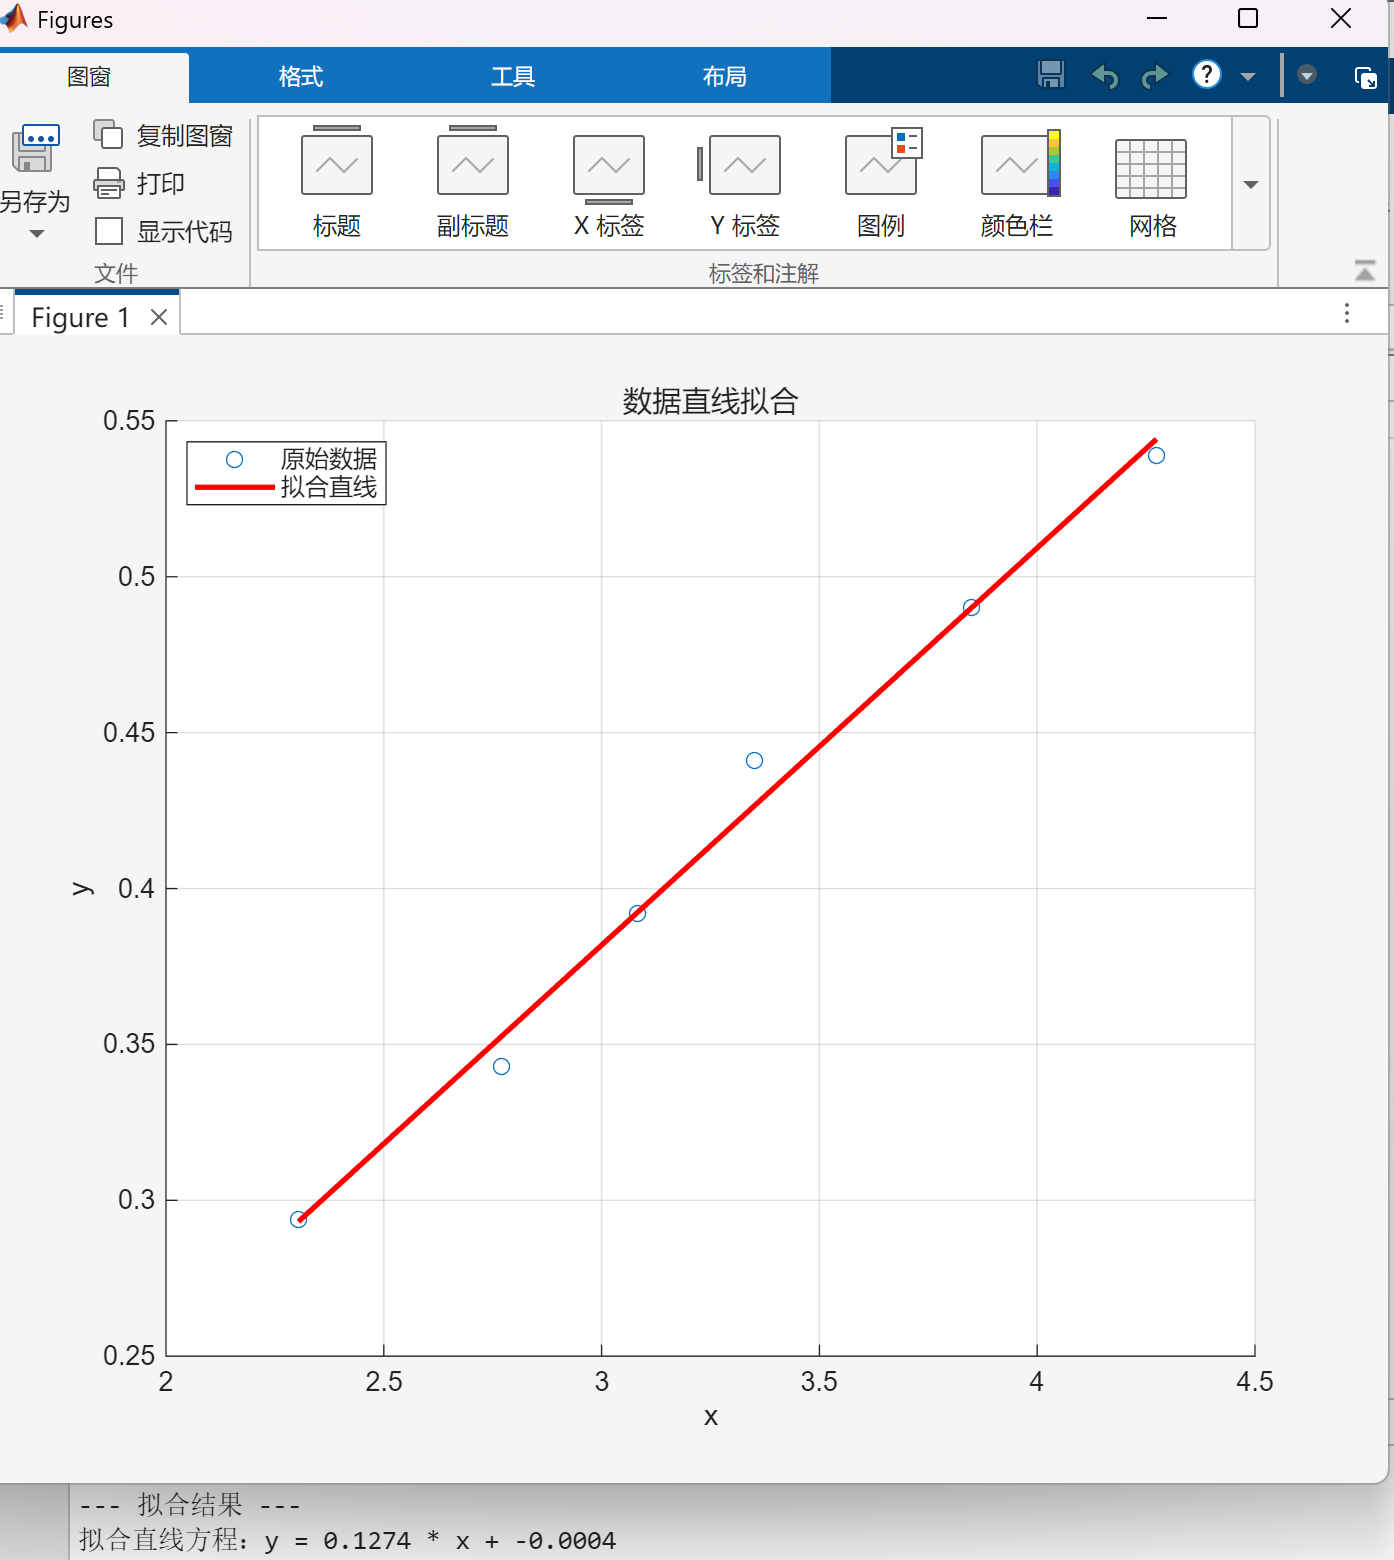
\includegraphics[width=0.6\textwidth]{figures/实验二数据拟合.png}
    \caption{实验二数据拟合图象}
\end{figure}
拟合结果：斜率 = 0.1274。斜率表示质量线密度，经过单位换算，$\rho = 1.274 \times 10^{-4} $(kg/m)

\subsection{误差分析（20分）}
（运用测量误差、相对误差或不确定度等分析实验结果，写出完整的结果表达式，并分析误差原因。）
\subsubsection{系统误差}
\textbf{(1)砝码质量：}砝码由于磨损/锈蚀等因素，其质量与5g/10g会有偏差。
\par
\textbf{(2)弦线非绝对均匀：}弦线不均匀会导致局部$\rho$与整体$\rho$的差异。
\par
\textbf{(3)振动源频率：}振动源可能存在频率不稳定（如电源电压波动）的问题。

\subsubsection{测量误差}
\textbf{(1)波长 $\lambda$ 的测量误差：}肉眼判断波节中心位置易受视觉偏差影响（尤其振幅较小时）；未形成稳定驻波时过早读数，导致频率测量偏差；砝码未稳定就读数（附加振动干扰）。
\par
\textbf{(2)测量仪器：}使用米尺/游标卡尺时的估读误差或仪器精度限制。

\subsubsection{环境干扰}
空气流动使弦振动不稳定；温度变化导致弦线热胀冷缩；实验台震动干扰驻波形成。

\subsection{实验探讨（10分）}
（对实验内容、现象和过程的小结，不超过100字。）
\par
在记录实验数据时，由于$L_\text{左}$实在是太不方便测量了（仪器最左端磨损严重），我决定改测两段驻波中间结点位置，这样$|L_\text{左} - L_\text{左}|$ 即为半波长。然后实验一在计算$\rho$时，如果先计算出波速u，保留一定的小数位后，再代入公式求得质量线密度$\rho$，这么做会带来额外的误差。所以我是直接把频率f、波长$\lambda$，代入公式。
\par
通过本次实验，我学会了如何观察固定弦振动传播时形成的横驻波，了解了振动在弦上传播的规律，掌握了改变频率或弦张力测算均匀弦上横波传播速度u及弦线密度$\rho$的方法。

\section{思考题（10分）}
（解答教材或讲义或老师布置的思考题，请先写题干，再作答。）
\subsection{什么叫驻波,它形成的条件是什么?}
驻波是指两列频率相同、振幅相同、传播方向相反的相干波在同一直线上叠加后形成的一种特殊波动现象，其波形不随时间向前传播，仅表现为各质点在各自平衡位置附近做简谐振动，存在始终静止不动的“波节”和振动最强的“波腹”。
\par
\textbf{形成条件：}
\par
（1）相干波叠加：需有两列频率相同、振幅相同、传播方向相反的相干波（如弦振动实验中，入射波与固定端反射波）
\par
（2）边界条件匹配：弦的两端为固定端时，反射波在端点形成波节，因此弦长需满足为半波长的整数倍，此时可形成稳定驻波。

\subsection{如何用驻波法测量未知振源的频率?}
驻波法测量频率的核心是利用驻波的形成条件和波速公式。当两列频率相同、传播方向相反的相干波叠加时，会形成稳定驻波，其波形固定不动，存在等间距的波节和波腹。对于两端固定的弦线或空气柱，驻波的波长$\lambda$ 与介质长度 L 满足关系：
\[
L = n \times \frac{\lambda}{2} \quad \text{n 为波节数}
\]
\par
结合波速公式 $v = f \lambda$，可得频率 $f = \frac{v}{\lambda} = \frac{nv}{2L}$
\par
若已知波速 v（由介质决定），通过测量弦线长度 L 和驻波段数 n，可求得频率。
\subsection{本实验的误差主要来源在哪里?}
\textbf{驻波的观察与确定：}肉眼确定是否形成稳定的驻波具有较高的难度。尤其当振幅较小的时候，改变右侧节点位置，波形变化不明显，肉眼容易产生误判。

\end{fullreportonly}
\insertnotes
\end{document}